\documentclass[11pt,twocolumn]{article}
\usepackage{graphicx}
\usepackage{fullpage}
\usepackage{amsmath,amsthm,amsfonts,amssymb,amscd}
\usepackage{lipsum}
\usepackage{titlesec}
\usepackage{longtable}
\usepackage[top=0.7in,bottom=1in,left=0.85in,right=0.85in]{geometry}

% title formatting
\titleformat{\section}
{\centering\normalfont\scshape}{\thesection.}{1em}{}
\titleformat{\subsection}
{\centering\normalfont\scshape}{\thesubsection.}{1em}{}

% spacing between columns
\setlength{\columnsep}{2em}

%title setup
\title{\vspace{-1cm}Lab \#X: Title of lab here. \\[0.4cm]\large{PHY224H1 S | Winter 2020}\vspace{-0.5em}}
\author{First Last \and First Last}
\date{\vspace{-0.3em}\normalsize\today}

%%%%%%%%%%%%%%%%%%%%%%%%%%%%%%%%%%%
\begin{document}

% one column abstract
\twocolumn[
  \begin{@twocolumnfalse}
    \maketitle
    \begin{abstract}
        Purpose. Key result. Most significant point of discussion. Major conclusion. \vspace{1.5em}
    \end{abstract}
  \end{@twocolumnfalse}
]

\section{Introduction}
\lipsum[1-1]

\subsection{Subsec 1}
\lipsum[2-3]

\subsection{Subsec 2}
\lipsum[3-5]

\section{Log and Data}
asdf sadf asdf asdf\hspace{0.2em}\footnote{\hspace{0.7em}testing footnotes} asdfasdfasdfa asdf asdf asdf 

\section{Questions and Analysis}
\lipsum[1-5]


\begin{table}[htb]
    \caption{\label{tab:table1}table table table label.}
    \vspace{1em}\hline\hline\vspace{0.3em}\centering
    \begin{tabular}{ccc}
        &$r_c$ (\AA)&$r_0$ (\AA)\\
        \hline
        Cu& 0.800 & 14.10\\
        Ag& 0.990 & 15.90\\
        Tl& 0.480 & 18.90\\
    \end{tabular}
    \hline\hline
\end{table}

asdfasdf

\section{Discussions/Conclusions}
\lipsum[1-3]


\begin{figure}[htb]
    \centering 
    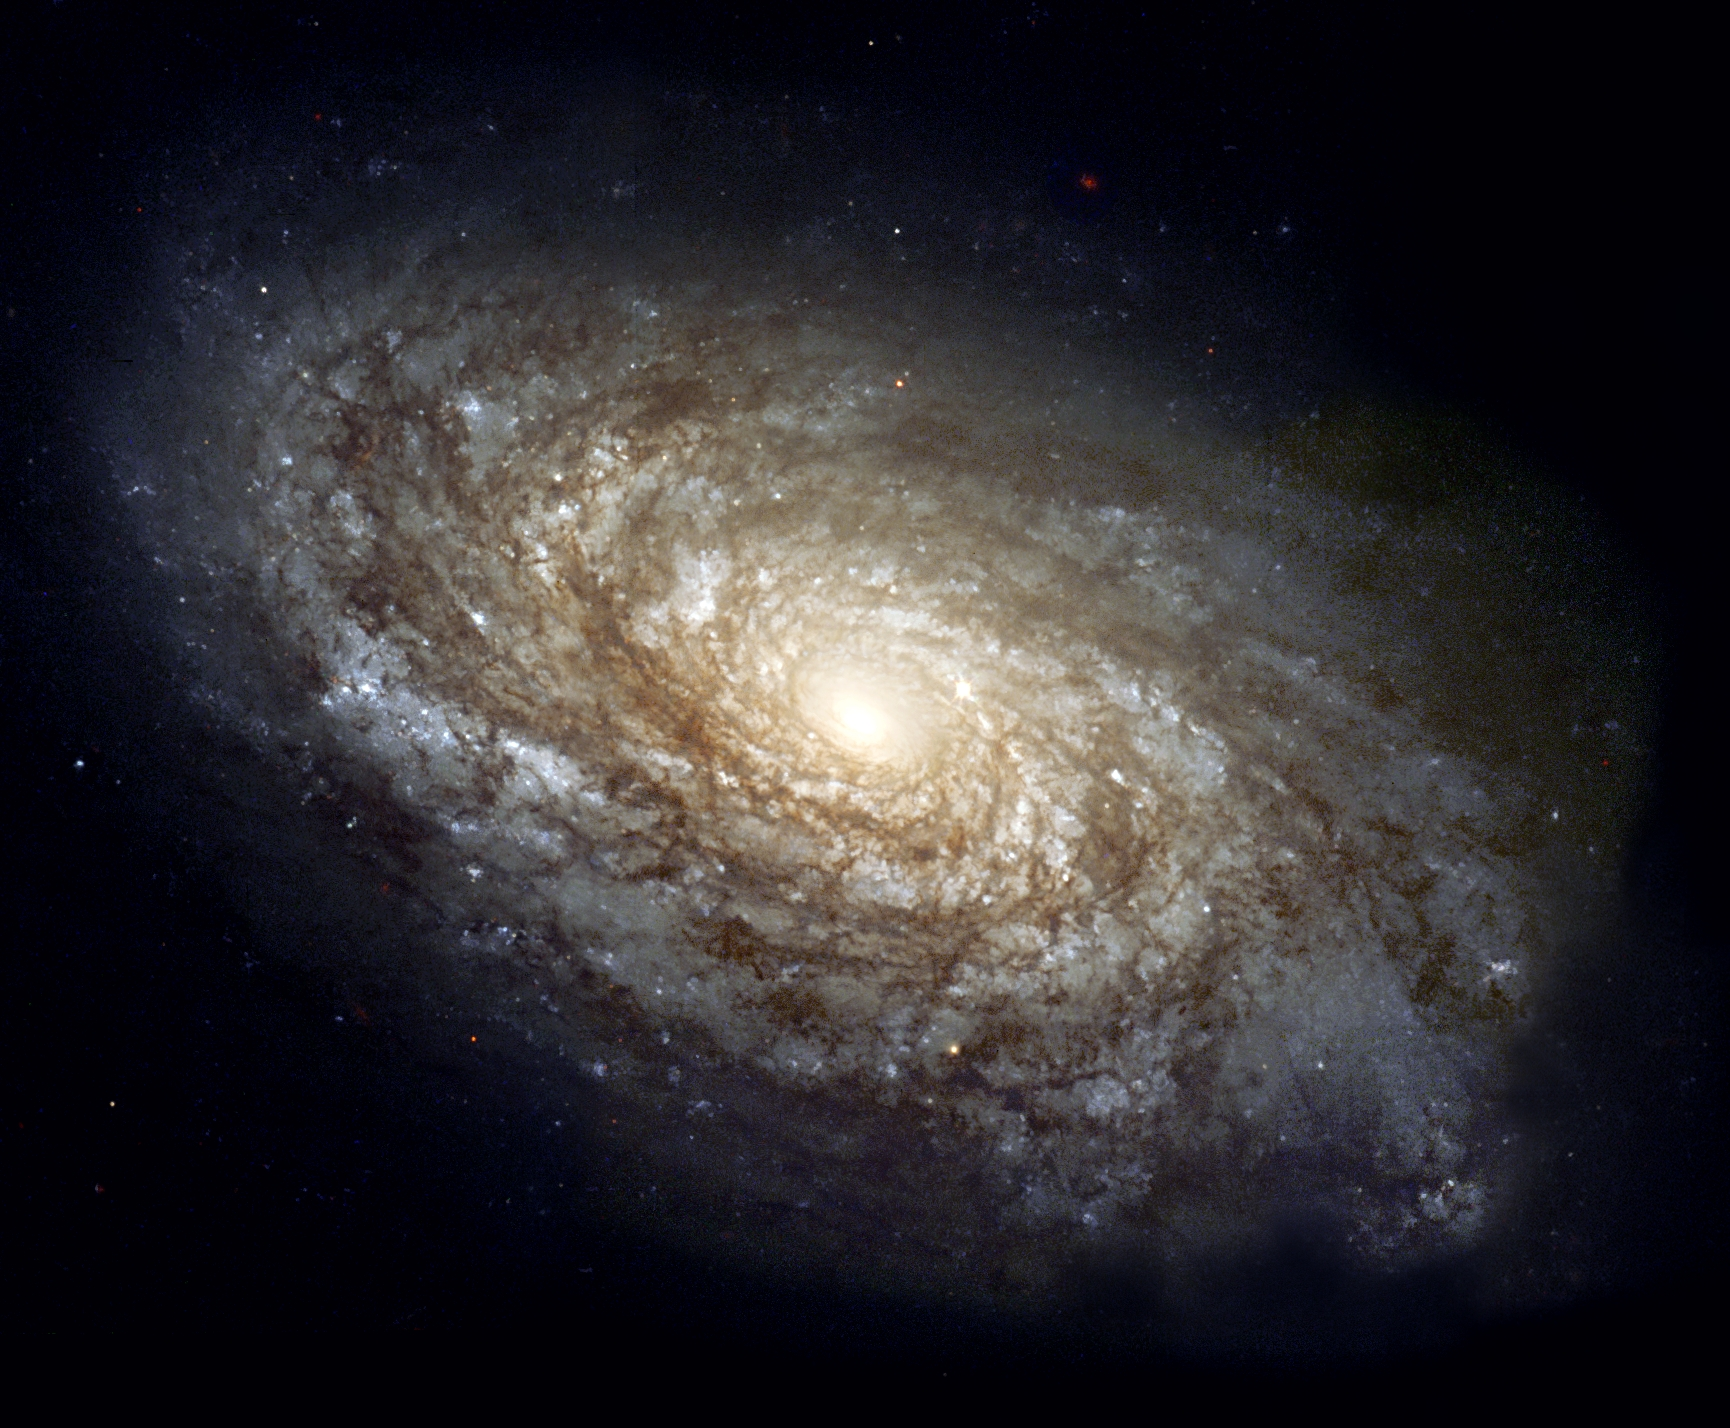
\includegraphics[width=\linewidth]{samplefig.jpg}
    \caption{\label{fig:galaxy}figure figure label}
\end{figure}

\lipsum[4-5]

\section{Computational Analysis}
\lipsum[1-5]

\end{document}
